\documentclass{standalone}
\usepackage{tikz}
\usepackage{amsmath}

\begin{document}

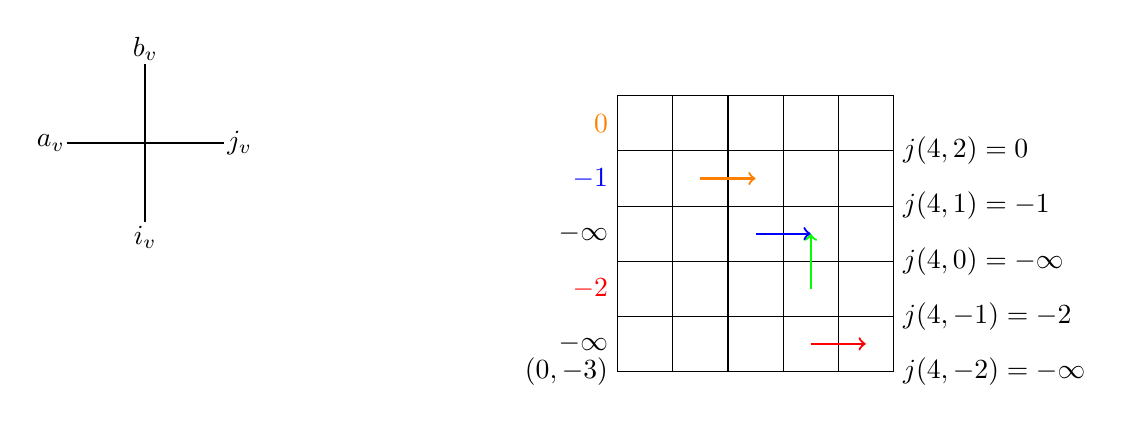
\begin{tikzpicture}

% Left diagram
\begin{scope}[xshift=-3cm]
    \draw[thick] (-1,0) -- (1,0);
    \draw[thick] (0,-1) -- (0,1);
    \node at (-1.2,0) {$a_v$};
    \node at (1.2,0) {$j_v$};
    \node at (0,-1.2) {$i_v$};
    \node at (0,1.2) {$b_v$};
\end{scope}

% Right grid and arrows
\begin{scope}[xshift=3cm, yshift=-1.5cm, scale=0.7]
    \foreach \x in {0,1,2,3,4} {
        \foreach \y in {-2,-1,0,1,2} {
            \draw (\x,\y) rectangle (\x+1,\y+1);
        }
    }
    
    % Arrows with colors
    \draw[thick, ->, green] (3.5,-0.5) -- ++(0,1);
    \draw[thick, ->, blue] (2.5,0.5) -- ++(1,0);
    \draw[thick, ->, orange] (1.5,1.5) -- ++(1,0);
    \draw[thick, ->, red] (3.5,-1.5) -- ++(1,0);
    
    % Labels
    \node[anchor=east] at (0,-2) {$(0,-3)$};
    \node[anchor=west] at (5,-2) {$j(4,-2) = -\infty$};
    \node[anchor=west] at (5,-1) {$j(4,-1) = -2$};
    \node[anchor=west] at (5,0) {$j(4,0) = -\infty$};
    \node[anchor=west] at (5,1) {$j(4,1) = -1$};
    \node[anchor=west] at (5,2) {$j(4,2) = 0$};
    
    % Color indicators on the left
    \node[anchor=east, orange] at (0,2.5) {$0$};
    \node[anchor=east, blue] at (0,1.5) {$-1$};
    \node[anchor=east] at (0,0.5) {$-\infty$};
    \node[anchor=east, red] at (0,-0.5) {$-2$};
    \node[anchor=east] at (0,-1.5) {$-\infty$};
\end{scope}

\end{tikzpicture}

\end{document}